\chapter{Pruebas y Resultados}\label{ch:pruebasyresultados}

La naturaleza del algoritmo propuesto hace difícil determinar la configuración
inicial del mismo ya que la forma de encontrar la máxima efectividad del mismo es
mediante la experimentación con distintos valores de sus parámetros.

Por este motivo se hace necesario realizar un conjunto de experimento que
permitan entender la influencia de los parámetros en el desempeño del algoritmo.
En particular analizaremos la influencia de:

\begin{itemize}
  \item Número de intentos al realizar el cruzamiento.
  \item Número de individuos del torneo.
  \item Número de intentos de mutación.
  \item Profundidad máxima del método grow.
  \item Profundidad máxima en el cruzamiento.
  \item Profundidad máxima en la mutación.
  \item Factor Fitness
\end{itemize}
 

En cada caso ejecutaremos el algoritmo dejando fijo el resto de parámetros y
modificando el parámetro bajo estudio. Al tratarse de procesos aleatorios cada
ejecución con la misma configuración puede ser completamente diferente, sin
embargo, al hacer la media de varias ejecuciones, podremos sacar conclusiones
objetivas sobre el rendimiento del algoritmo con la configuración. Por esto, se
procede a lanzar 10 ejecuciones de cada configuración. Después  de las
ejecuciones analizaremos la media de los resultados para compararla con la media
de otras ejecuciones.

\section{Número de intentos al realizar
cruzamiento}\label{sec:p-intentos-cruzamiento}

Como se describe en la sección \ref{para:crossover}, a la hora de realizar el
cruzamiento se pueden permitir una serie de intentos para obtener un árbol
válido. En caso de que no se obtenga un árbol válido en el número de intentos
especificados, no se llevará a cabo el cruzamiento. Con este experimento queremos
determinar cual es el valor más conveniente para el problema que nos hemos
planteado.

\begin{table}[tb]
\caption{Valores de los parámetros para el número de intentos al realizar el
cruzamiento.}
\label{tab:cross-tries}
\centering
\begin{tabular}{lcccc}
\toprule
  &\textbf{Prueba 1} & \textbf{Prueba 2} & \textbf{Prueba 3} &\textbf{Prueba
  4}\\
\midrule
gp.koza.xover.tries    & $1$ & $10$ & $100$ & $1000$ \\
\bottomrule
\end{tabular}
\end{table}


En la tabla \ref{tab:cross-tries} se encontrarán los valores de los parámetros
que se han utilizado para este caso. La figura \ref{subfig:p-crosstries-best}
muestra la evolución de los valores de fitness del mejor individuo a través de
las distintas iteraciones para los distintos valores del parámetro analizado. De
manera similar la figura \ref{subfig:p-crosstries-mean} presenta los valores que
toma el fitness medio de la población a medida que avanza la ejecución del
algoritmo. Como complemento a las figuras anteriores, en la figura
\ref{subfig:p-crosstries-nodes} se puede apreciar el número medio de nodos de los
árboles de programa de la población. Finalmente la figura
\ref{subfig:p-crosstries-time}  se refiere al consumo de recursos
computacionales durante la ejecución del programa.


El análisis de las figuras anteriores nos permite concluir que la cantidad de
intentos (verde) resulta más conveniente porque produce el mejor desempeño, y
además se puede observar que el valor del parámetro no implica mayores costes
computacionales que otros de peor calidad.

Resulta interesante constatar que el número de nodos se mantiene en rangos
similares en la primera parte de la ejecución del algoritmo pero a partir de un
punto empiezan a divergir.

Como resultado de este experimento podemos concluir que el valor más conveniente
de la cantidad de intentos para realizar con éxito el cruzamiento es $1000$
intentos.


\begin{figure}[cbt]
  \centering
  \subfloat[Calidad de los mejores individuos]{
  	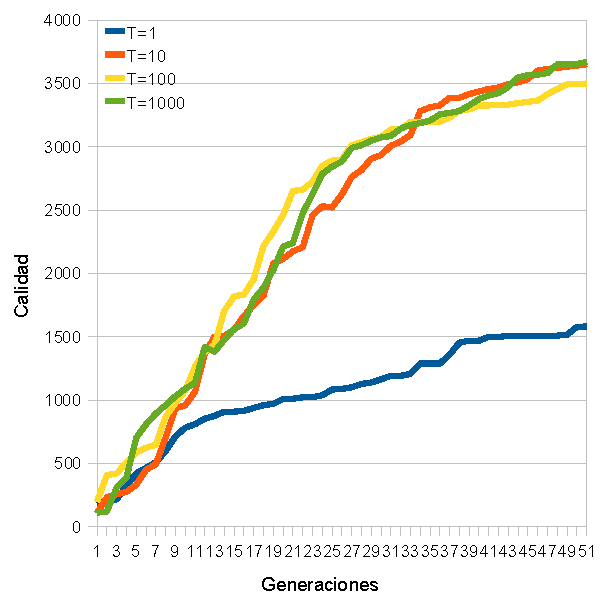
\includegraphics[width=0.4\textwidth]{figs/graphs/CrossTriesBest}
	\label{subfig:p-crosstries-best}
  }                
  \subfloat[Calidad media de la población]{
  	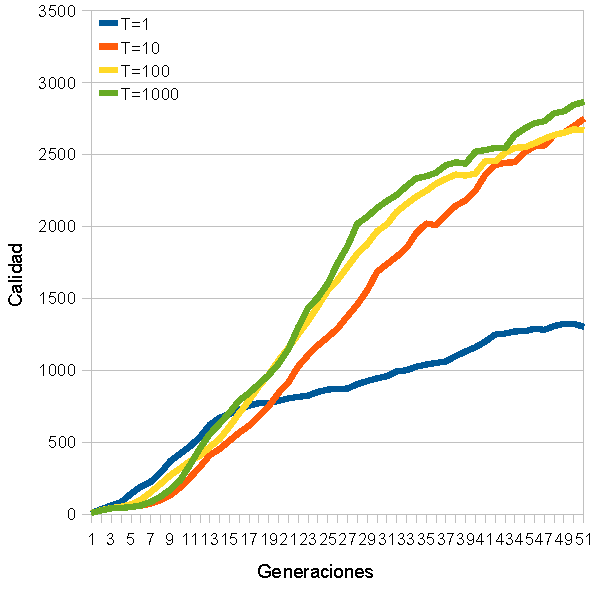
\includegraphics[width=0.4\textwidth]{figs/graphs/CrossTriesMean}
	\label{subfig:p-crosstries-mean}%
  }
  \quad
  \subfloat[Número de nodos medio de la población]{
  	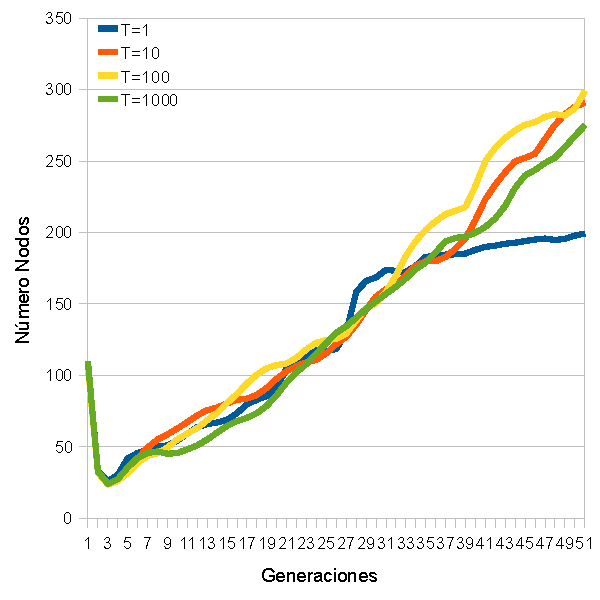
\includegraphics[width=0.4\textwidth]{figs/graphs/CrossTriesNodes}
	\label{subfig:p-crosstries-nodes}%
  }
  \subfloat[Tiempo de las ejecuciones]{
  	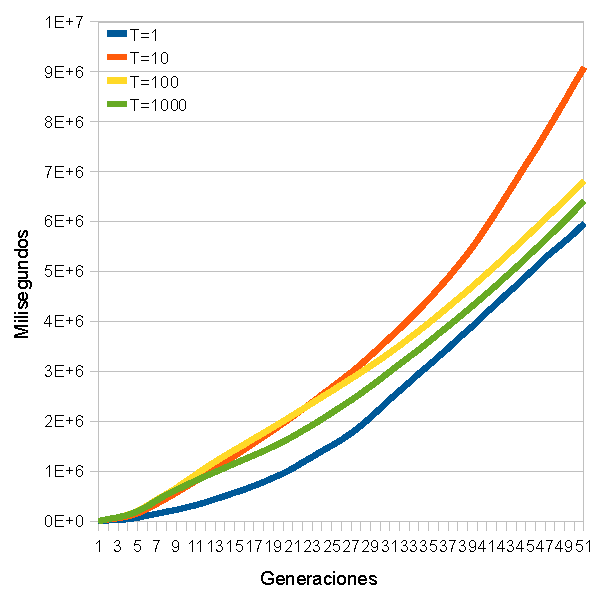
\includegraphics[width=0.4\textwidth]{figs/graphs/CrossTriesTime}
	\label{subfig:p-crosstries-time}%
  }
  \centering
\caption{Número de intentos de realizar
cruzamiento ($T$)}
\label{fig:p-crosstries}
\end{figure}

%  
\section{Número de individuos del torneo}\label{sec:p-individuos-torneo}

El número de individuos del torneo, descrito en la sección Y, es el número de
individuos que entran en el torneo de selección del padre y la madre para
producir un nuevo individuo.

El resultado esperado es que, al aumentar el número, la probabilidad de escoger
al individuo más apto es mayor. De esta forma, el individuo más apto ganará
siempre los torneos, distribuyendo su código genético en la siguiente generación.
Por ello, la diversidad de la población disminuirá.

Por el contrario, si el número de individuos en el torneo es muy bajo, las
probabilidades de que en el torneo aparezcan individuos más aptos es menor. Por
ello, es posible que se pierdan individuos muy aptos que deberían haber tenido
descendencia.

\begin{table}[cbt]
\caption{Valores de los parámetros para el número de individuos del torneo.}
\label{tab:individuos-torneo}
\centering
\begin{tabular}{lccc}
\toprule
  &\textbf{Prueba 5} & \textbf{Prueba 6} & \textbf{Prueba 7}\\
\midrule
select.tournament.size &  $2$  & $4$ & $7$ \\
\bottomrule
\end{tabular}
\end{table}


Siguiendo la estructura presentada en la sección \ref{sec:p-individuos-torneo}
(tabla de parámetros \ref{tab:individuos-torneo}) tanto la figura
\ref{subfig:p-tournsize-best} que muestra la calidad media como la figura \ref{subfig:p-tournsize-mean} que muestra la calidad máxima, nos
indican que el mejor desempeño lo ofrece el valor 4 para el número de individuos
del torneo. Este hecho confirma nuestra previsión de los resultados, ya que un
valor bajo como 2 ofrece muy poco rendimiento, y un valor alto como 7 no supera
la calidad obtenida por el valor 4.

El número de nodos (figura \ref{subfig:p-tournsize-nodes}) nos índica que
el valor 2 produce árboles con pocos nodos, el valor 4 produce árboles de tamaño
medio y el valor 7 produce los árboles con un mayor número de nodos. En este
caso, la exigencia computacional (figura \ref{subfig:p-tournsize-time}) va a la
par del número de nodos.


\begin{figure}[cbt]
  \centering
  \subfloat[Calidad de los mejores individuos]{
  	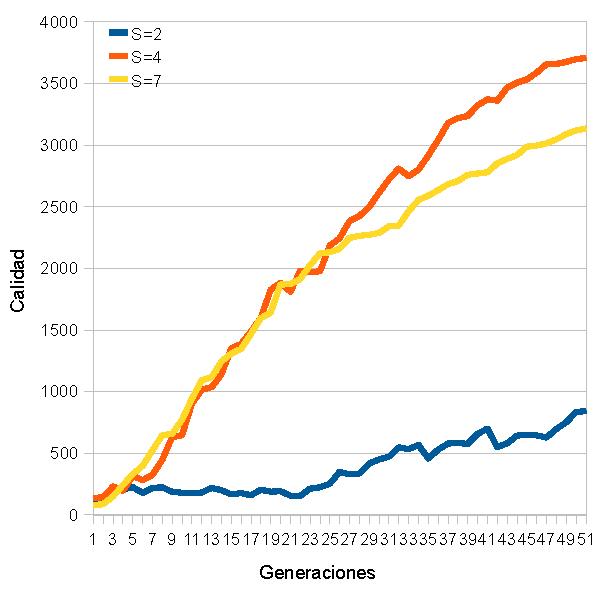
\includegraphics[width=0.4\textwidth]{figs/graphs/TournSizeBest}
	\label{subfig:p-tournsize-best}
  }                
  \subfloat[Calidad media de la población]{
  	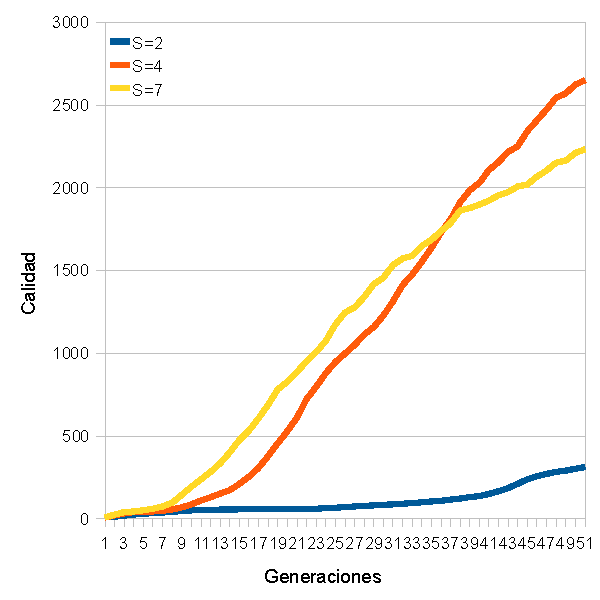
\includegraphics[width=0.4\textwidth]{figs/graphs/TournSizeMean}
	\label{subfig:p-tournsize-mean}%
  }
  \quad
  \subfloat[Número de nodos medio de la población]{
  	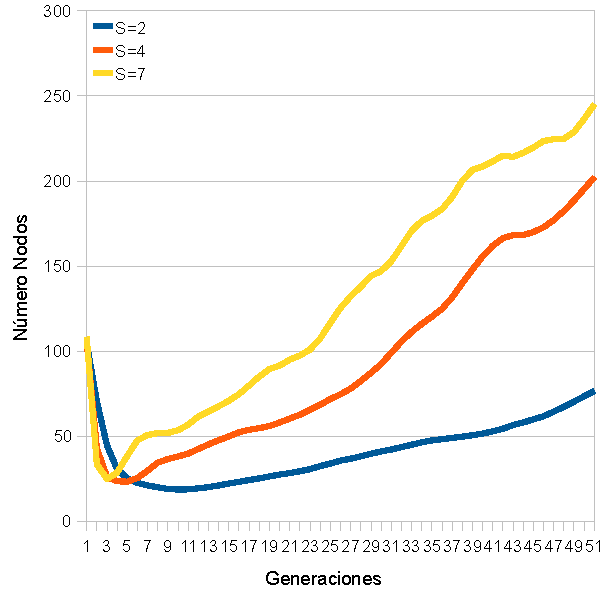
\includegraphics[width=0.4\textwidth]{figs/graphs/TournSizeNodes}
	\label{subfig:p-tournsize-nodes}%
  }
  \subfloat[Tiempo de las ejecuciones]{
  	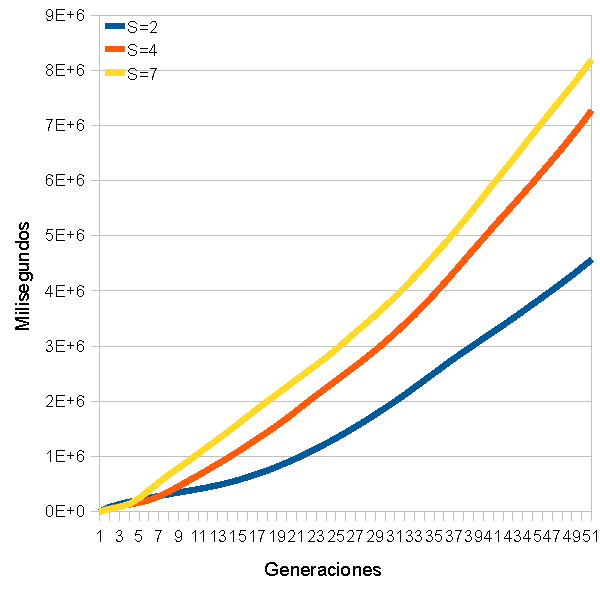
\includegraphics[width=0.4\textwidth]{figs/graphs/TournSizeTime}
	\label{subfig:p-tournsize-time}%
  }
  \centering
\caption{Número de individuos del torneo ($S$)}
\label{fig:p-crosstries}
\end{figure}


\section{Número de intentos de mutación}\label{sec:p-intentos-mutacion}

El número de intentos de mutación es el número de intentos del algoritmo para
generar una mutación válida en el árbol de programa, donde una mutación válida es
aquella que consigue generar un árbol sintácticamente correcto. En nuestro
algoritmo, la mutación seleccionará un punto en el árbol aleatoriamente y
generará un subárbol también aleatoriamente.

El número de intentos de mutación representa la probabilidad de mutación. Así, 0
significa que no existirá mutación; 1 que hay mutación pero con muy baja
probabilidad. Sin embargo, no podemos asegurar nunca un 100\% de probabilidad de
mutación, ya que siempre es posible superar un número de intentos (por alto que
sea) sin encontrar una mutación válida.

\begin{table}[tb]
\caption{Valores de los parámetros para el número de intentos de mutación.}
\label{tab:mutate-tries}
\centering
\begin{tabular}{lccc}
\toprule
  &\textbf{Prueba 8} & \textbf{Prueba 9} & \textbf{Prueba 10}\\
\midrule
gp.koza.mutate.tries & $0$ &  $1$  & $10$ \\
\bottomrule
\end{tabular}
\end{table}

Una vez realizadas las pruebas con los valores indicados en la tabla
\ref{tab:mutate-tries}, los resultados revelan que el mejor desempeño (figuras
\ref{subfig:p-mutatetries-best} y \ref{subfig:p-mutatetries-mean}) se encuentra
cuando el número de intentos de mutación es 10. Además es posible que un valor
más elevado pueda conseguir mejor desempeño, sin embargo, para ser un estudio
científico riguroso tendríamos que realizar otro estudio en detalle para
optimizar este parámetro.

La mejora del rendimiento (figura \ref{subfig:p-mutatetries-time}) debido al
aumento de la probabilidad de mutación puede deberse a que al principio del proceso evolutivo aparece una reducción general de
nodos (figura \ref{subfig:p-mutatetries-nodes} generaciones 1-4) y por ello la
diversidad se reduce. La mutación  es un operador que aporta nueva diversidad a
la población en cualquier punto de la evolución. Por ello creemos que la mutación
es necesaria para la evolución en este problema, y, no obstante, probablemente
exista un límite superior donde la mutación no beneficie a la calidad de los
individuos.

\begin{figure}[cbt]
  \centering
  \subfloat[Calidad de los mejores individuos]{
  	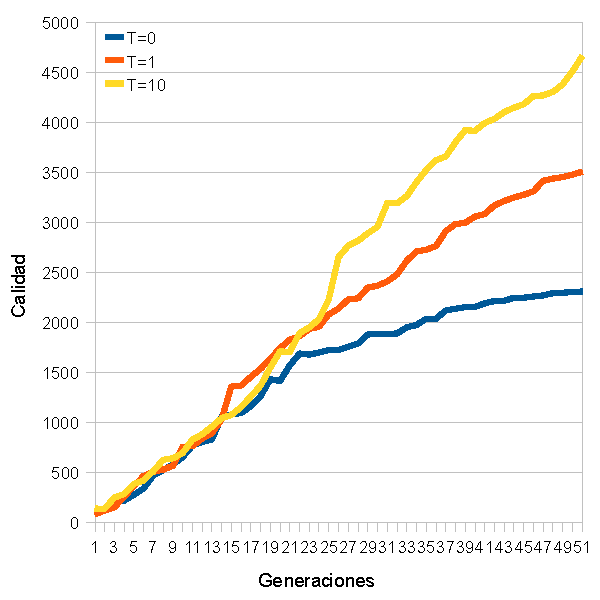
\includegraphics[width=0.4\textwidth]{figs/graphs/MutateTriesBest}
	\label{subfig:p-mutatetries-best}
  }                
  \subfloat[Calidad media de la población]{
  	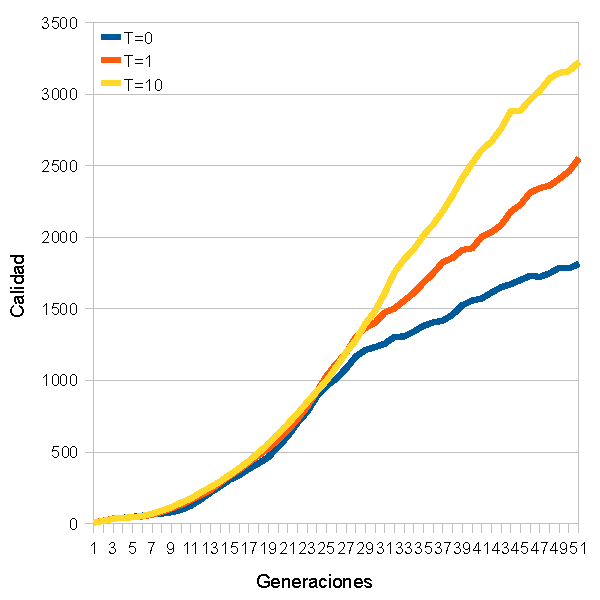
\includegraphics[width=0.4\textwidth]{figs/graphs/MutateTriesMean}
	\label{subfig:p-mutatetries-mean}%
  }
  \quad
  \subfloat[Número de nodos medio de la población]{
  	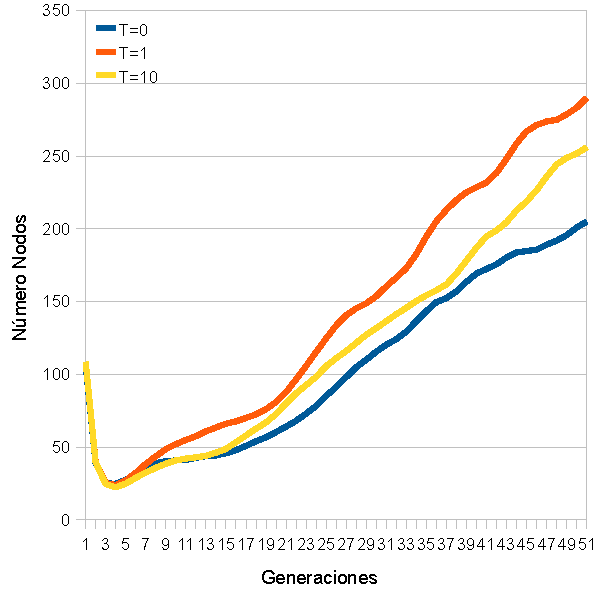
\includegraphics[width=0.4\textwidth]{figs/graphs/MutateTriesNodes}
	\label{subfig:p-mutatetries-nodes}%
  }
  \subfloat[Tiempo de las ejecuciones]{
  	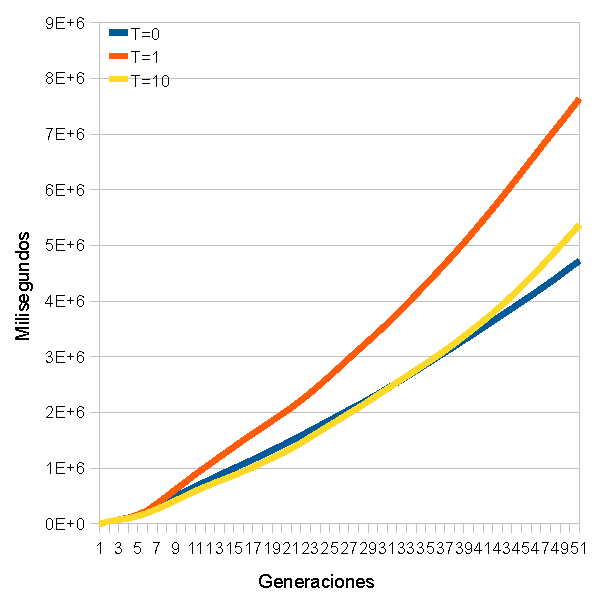
\includegraphics[width=0.4\textwidth]{figs/graphs/MutateTriesTime}
	\label{subfig:p-mutatetries-time}%
  }
  \centering
\caption{Número de intentos de mutación ($T$)}
\label{fig:p-crosstries}
\end{figure}


\section{Profundidad máxima del método grow}\label{sec:p-prof-grow}

La profundidad máxima del método grow afecta a los árboles generados por este
método. Este método sólo se utiliza al inicializar la población, por lo que en
principio solo debería afectar al inicio del algoritmo.

\begin{table}[cbt]
\caption{Valores de la profundidad máxima del método grow.}
\label{tab:prof-grow}
\centering
\begin{tabular}{lcc}
\toprule
  &\textbf{Prueba 11} & \textbf{Prueba 12}\\
\midrule
gp.koza.grow.max-depth & $10$ & $100$  \\
\bottomrule
\end{tabular}
\end{table}

Siguiendo la línea de las secciones anteriores y la tabla de datos
\ref{tab:prof-grow}, las figuras \ref{subfig:p-growdepth-best} y
\ref{subfig:p-growdepth-mean} muestran la evolución de nuestro algoritmo en el
tiempo y las figuras \ref{subfig:p-growdepth-nodes} y
\ref{subfig:p-growdepth-time} muestran la evolución del número de nodos y el
rendimiento del algorítmo respectivamente. Para esta prueba no muestran
información relevante ya que en ambas pruebas se percibe un desempeño parecido.
No obstante, parece que el valor 100 mejora ligeramente la calidad de los
individuos, aunque es posible que se trate de un evento casual (recordemos cada
ejecución se comporta de forma diferente debido a aleatoriedad del algoritmo).

\begin{figure}[tb]
  \centering
  \subfloat[Calidad de los mejores individuos]{
  	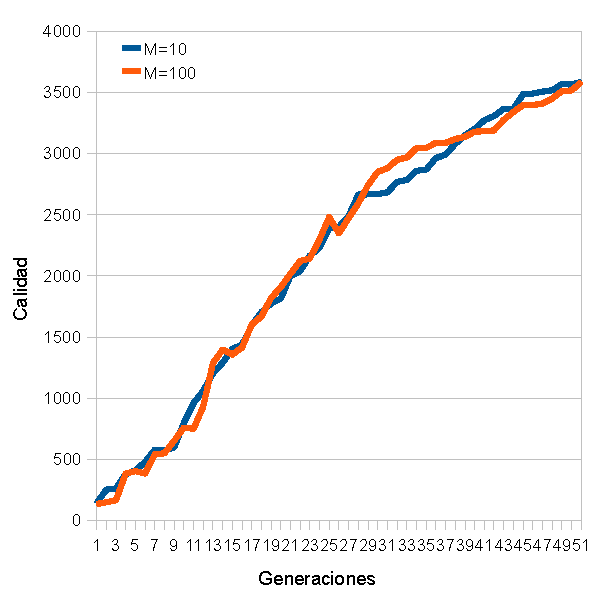
\includegraphics[width=0.4\textwidth]{figs/graphs/GrowMaxBest}
	\label{subfig:p-growdepth-best}
  }                
  \subfloat[Calidad media de la población]{
  	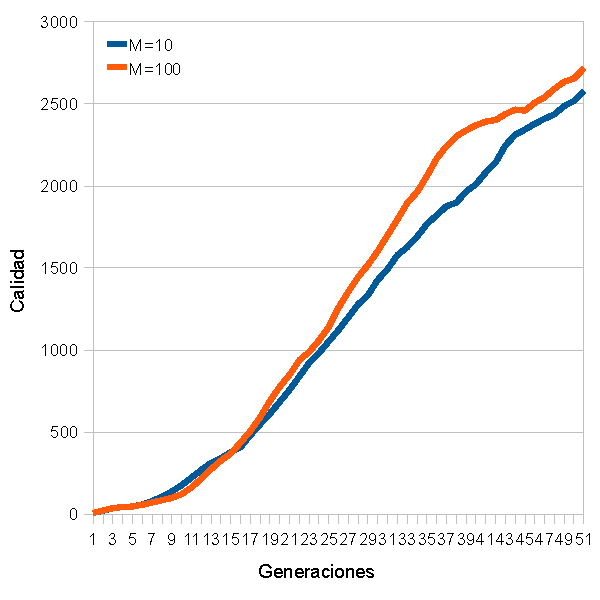
\includegraphics[width=0.4\textwidth]{figs/graphs/GrowMaxMean}
	\label{subfig:p-growdepth-mean}%
  }
  \quad
  \subfloat[Número de nodos medio de la población]{
  	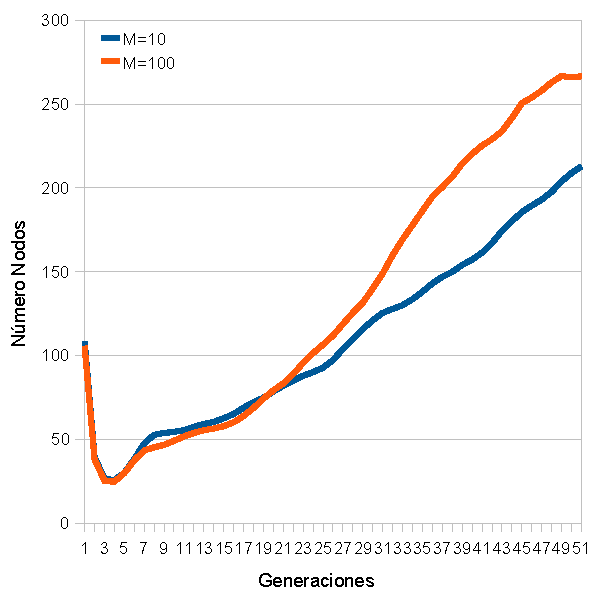
\includegraphics[width=0.4\textwidth]{figs/graphs/GrowMaxNodes}
	\label{subfig:p-growdepth-nodes}%
  }
  \subfloat[Tiempo de las ejecuciones]{
  	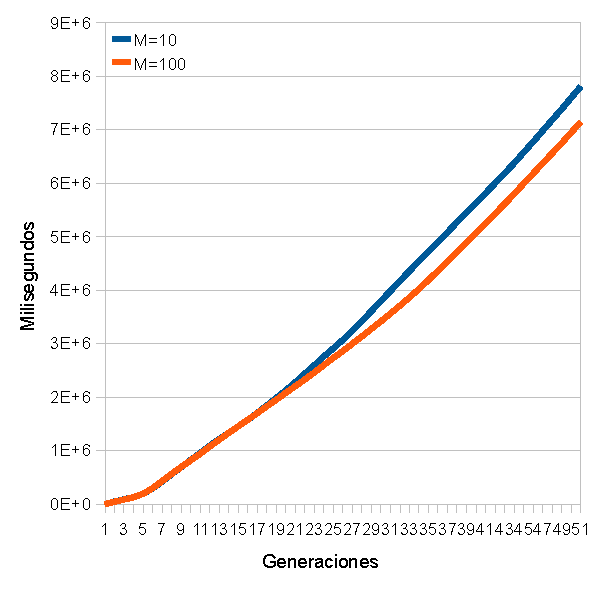
\includegraphics[width=0.4\textwidth]{figs/graphs/GrowMaxTime}
	\label{subfig:p-growdepth-time}%
  }
  \centering
\caption{Profundidad máxima del método grow ($M$)}
\label{fig:p-crosstries}
\end{figure}


\section{Profundidad máxima en el cruzamiento}\label{sec:p-prof-cross}

El parámetro de la profundidad máxima de cruzamiento se utilizará en el
cruzamiento de individuos e indica la profundidad máxima que tendrá el subárbol
seleccionado para ser intercambiado.

\begin{table}[tb]
\caption{Valores de los parámetros para la profundidad máxima en el
cruzamiento.}
\label{tab:prof-cross}
\centering
\begin{tabular}{lcc}
\toprule
  &\textbf{Prueba 13} & \textbf{Prueba 14}\\
\midrule
gp.koza.xover.maxdepth $30$ & $100$  \\
\bottomrule
\end{tabular}
\end{table}


Como indica claramente la figura \ref{subfig:p-maxdepthcross-best} y
\ref{subfig:p-maxdepthcross-mean} en el desempeño de los datos de la tabla
\ref{tab:prof-cross}, el mejor rendimiento se obtiene cuando la profundidad
máxima es menor, en concreto 17. Además se puede observar que el número de nodos
(figura \ref{subfig:p-maxdepthcross-nodes}) es mayor a lo largo del tiempo cuando
la profundidad máxima es mayor. Esto es debido cuanta más profundidad, mayor es
el número de nodos que intercambiamos. El rendimiento (figura
\ref{subfig:p-maxdepthcross-time}) muestra, fuera de lo esperado, una relación
indirectamente proporcional entre el tiempo y el número de nodos. Este evento
puede ser debido a que ambas pruebas albergan un número de nodos parecidos y
por ello, el rendimiento del arbol no depende únicamente del árbol de programa,
sino que influye la rapidez en la que se evaluan las condiciones del árbol. 


\begin{figure}[tb]
  \centering
  \subfloat[Calidad de los mejores individuos]{
  	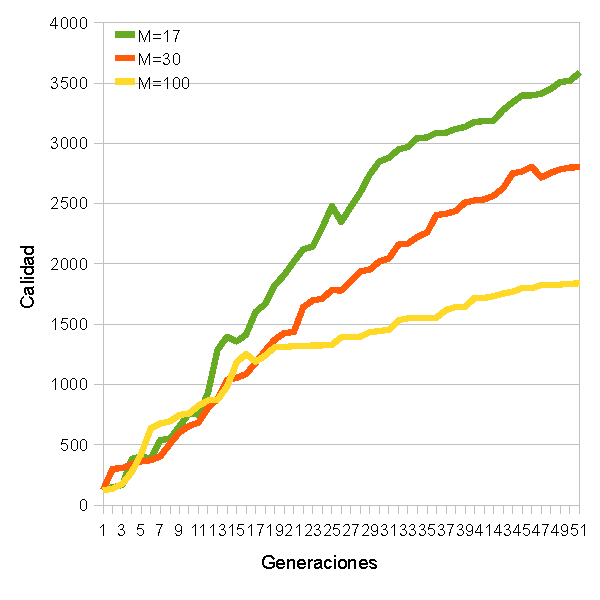
\includegraphics[width=0.4\textwidth]{figs/graphs/MaxDepthCrossBest}
	\label{subfig:p-maxdepthcross-best}
  }                
  \subfloat[Calidad media de la población]{
  	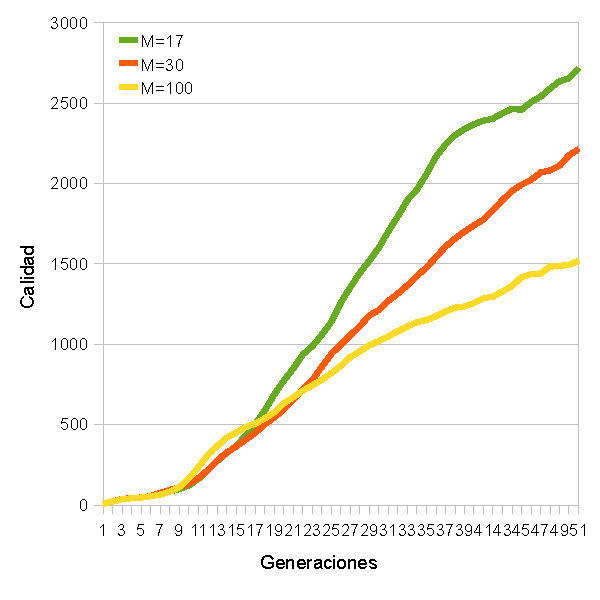
\includegraphics[width=0.4\textwidth]{figs/graphs/MaxDepthCrossMean}
	\label{subfig:p-maxdepthcross-mean}%
  }
  \quad
  \subfloat[Número de nodos medio de la población]{
  	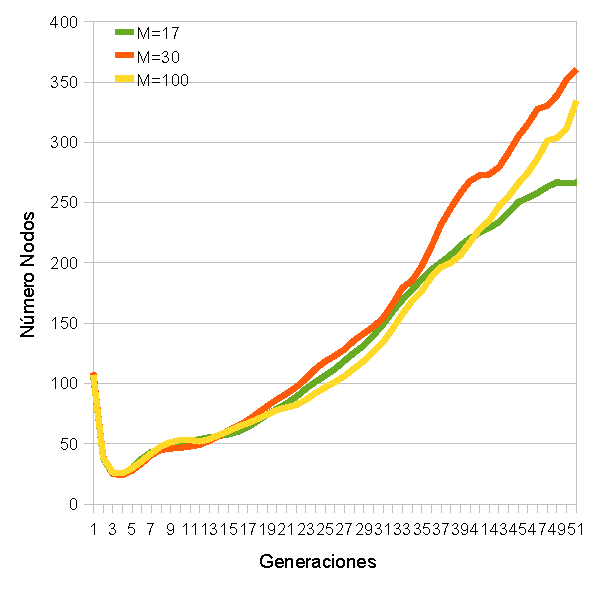
\includegraphics[width=0.4\textwidth]{figs/graphs/MaxDepthCrossNodes}
	\label{subfig:p-maxdepthcross-nodes}%
  }
  \subfloat[Tiempo de las ejecuciones]{
  	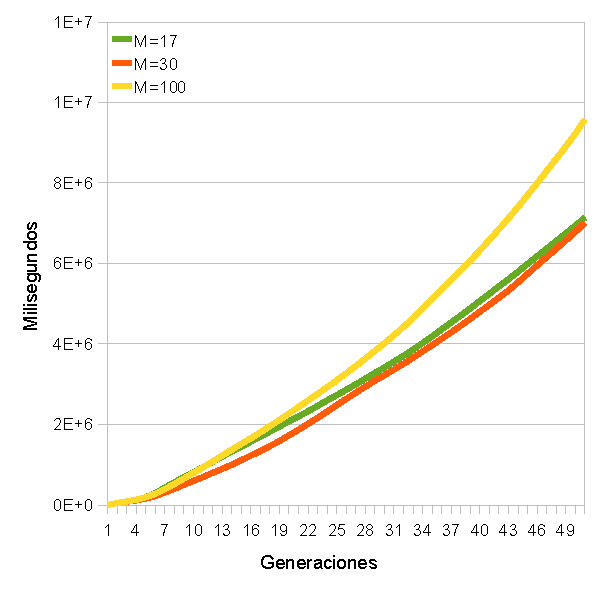
\includegraphics[width=0.4\textwidth]{figs/graphs/MaxDepthCrossTime}
	\label{subfig:p-maxdepthcross-time}%
  }
  \centering
\caption{Profundidad máxima en el cruzamiento ($M$)}
\label{fig:p-crosstries}
\end{figure}


\section{Profundidad máxima en la mutación}\label{sec:p-prof-mut}	

La profundidad máxima de mutación ajusta la longitud máxima que un subárbol
generado aleatoriamente podrá tener. Si el árbol excede esta profundidad, el
subárbol será descartado y se generará otro nuevo subárbol.

El comportamiento esperado es que según se aumenta la profundidad máxima, es más
probable que se generen árboles válidos, y, además, estos tendrán una longitud
mayor. En el caso que se disminuya la profundidad máxima, la mutación se
producirá con menos probabilidad y, en el caso de que aparezca el fenómeno, el
subárbol generado será de menor longitud.

\begin{table}[cbt]
\caption{Valores de los parámetros para la profundidad máxima en la mutación.}
\label{tab:prof-mut}
\centering
\begin{tabular}{lcc}
\toprule
  &\textbf{Prueba 15} & \textbf{Prueba 16}\\
\midrule
gp.koza.mutate.maxdepth & $30$ & $100$  \\
\bottomrule
\end{tabular}
\end{table}

Si observamos las gráficas de calidad (figura \ref{subfig:p-maxdepthmutate-best}
y \ref{subfig:p-maxdepthmutate-mean}) obtenidas mediante los parámetros de la
tabla \ref{tab:prof-mut}, observamos un fenómeno curioso. El mejor rendimiento
del algoritmo se encuentra cuando la profundad máxima es 17 y 100, sin embargo,
el peor desempeño lo tiene la ejecución con valor 30. La figura de número de
nodo \ref{subfig:p-mutatetries-nodes} y la figura del rendimiento
\ref{subfig:p-mutatetries-time} no indican ningún dato que resaltar.

Como el valor que mejor calidad ofrece es 100, optaremos por este valor de
configuración.


\begin{figure}[tb]
  \centering
  \subfloat[Calidad de los mejores individuos]{
  	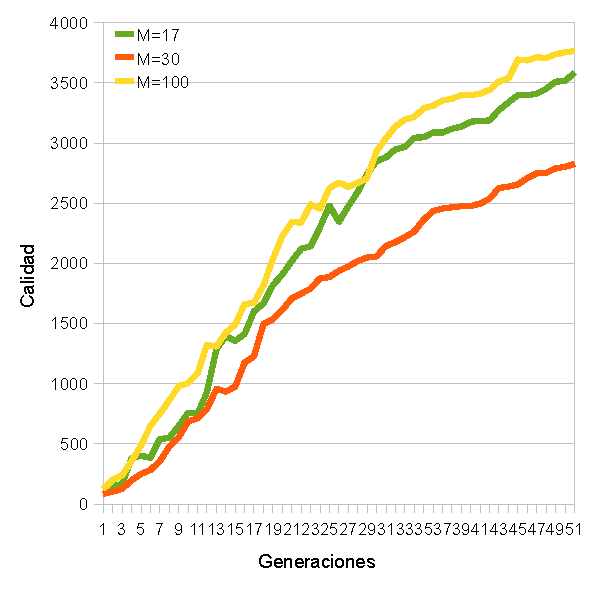
\includegraphics[width=0.4\textwidth]{figs/graphs/MaxDepthMutateBest}
	\label{subfig:p-maxdepthmutate-best}
  }                
  \subfloat[Calidad media de la población]{
  	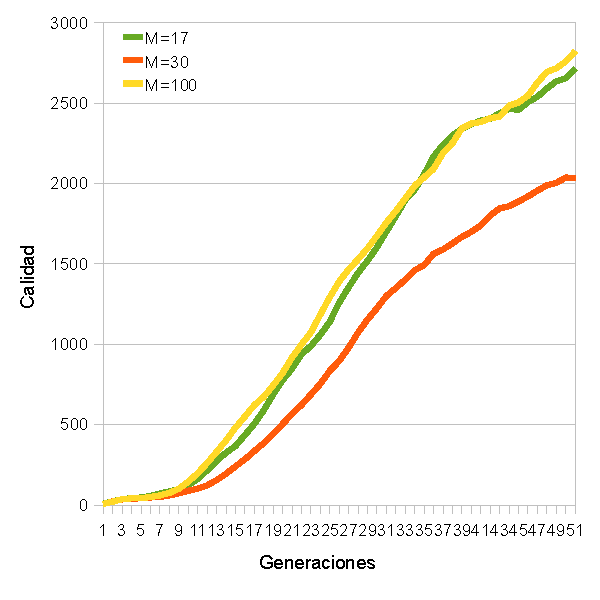
\includegraphics[width=0.4\textwidth]{figs/graphs/MaxDepthMutateMean}
	\label{subfig:p-maxdepthmutate-mean}%
  }
  \quad
  \subfloat[Número de nodos medio de la población]{
  	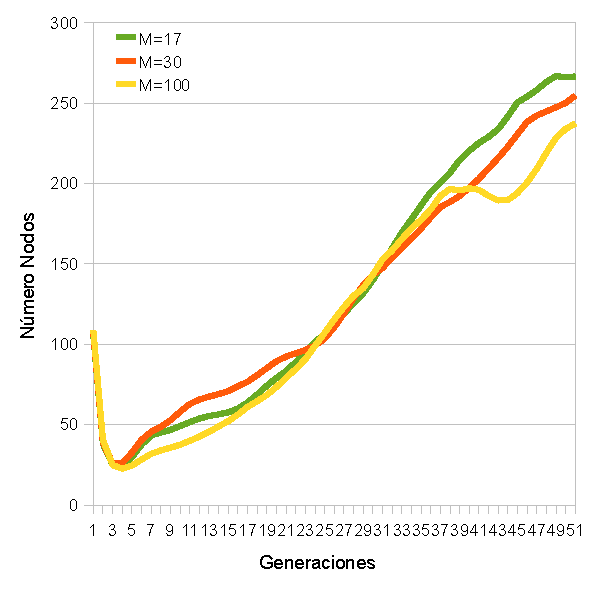
\includegraphics[width=0.4\textwidth]{figs/graphs/MaxDepthMutateNodes}
	\label{subfig:p-maxdepthmutate-nodes}%
  }
  \subfloat[Tiempo de las ejecuciones]{
  	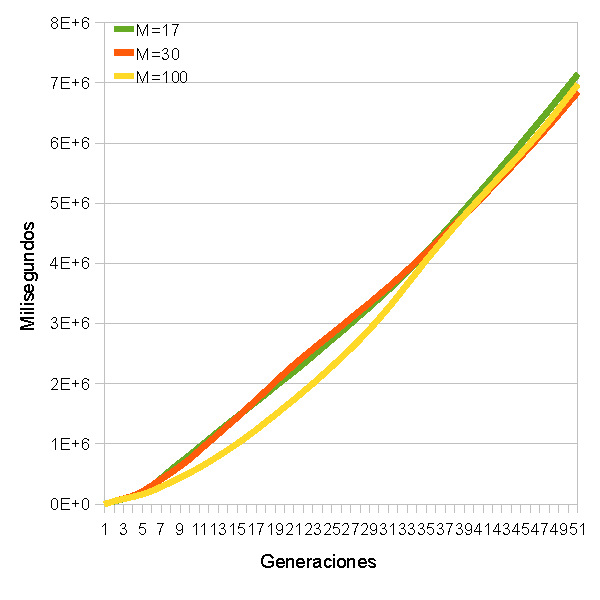
\includegraphics[width=0.4\textwidth]{figs/graphs/MaxDepthMutateTime}
	\label{subfig:p-maxdepthmutate-time}%
  }
  \centering
\caption{Profundidad máxima en la mutación ($M$)}
\label{fig:p-crosstries}
\end{figure}

\section{Factor fitness}\label{sec:p-factor-fitness}	

El factor del fitness es un valor que nos sirve para ponderar la suma de los
cubos resueltos de diferentes dificultades. De esta forma obtenemos una nota que
nos indica la calidad del individuo. La fórmula esta descrita en la sección
\ref{subsec:cubosresueltos}.

Un valor bajo, como 1, valora de la misma forma un cubo resuelto de nivel 1 que
de máximo, de tal forma que 10 cubos fáciles resueltos valen la misma puntuación
que 10 cubos difíciles resueltos. El único objetivo del algoritmo es resolver el
máximo número de cubos posibles independientemente de su dificultad.

Un valor más alto a 1, guía al proceso evolutivo a intentar resolver cubos de
mayor de dificultad ignorando los de menor dificultad. Así si el factor es 2, y
se resuelve un cubo de nivel 2, tendremos una puntuación de 4, y si otro
individuo resuelve 3 cubos de nivel uno, vencerá al individuo que resolvía uno de
nivel 2. De esta forma, cuanto más alto sea el valor del factor, mayor es la
importancia que tiene resolver un cubo de mayor dificultad.

Como el valor del fitness no es equiparable en cada prueba, compararemos las
pruebas con el valor medio de la entropía de cubos resueltos. De esta forma
podremos equiparar el desempeño de cada prueba.

\begin{table}[tb]
\caption{Valores de los parámetros para el factor del fitness.}
\label{tab:factor-fitness}
\centering
\begin{tabular}{lccc}
\toprule
  &\textbf{Prueba 17} & \textbf{Prueba 18} & \textbf{Prueba 19}\\
\midrule
gp.koza.fitness.factorfitness & $1$ & $2$ & $4$   \\
\bottomrule
\end{tabular}
\end{table}

En contra de lo que pensábamos, el resultado de las pruebas (figura
\ref{fig:p-factorfitness}) de los datos expuestos en la tabla
\ref{tab:factor-fitness} nos indica que el mejor rendimiento se obtiene cuando el
valor del factor es 1. Esto puede ser debido a que el sistema aprende a resolver
los casos básicos y lentamente va resolviendo casos más complicados.

\begin{figure}[tb]
  \centering
  \subfloat[Calidad de los mejores individuos]{
  	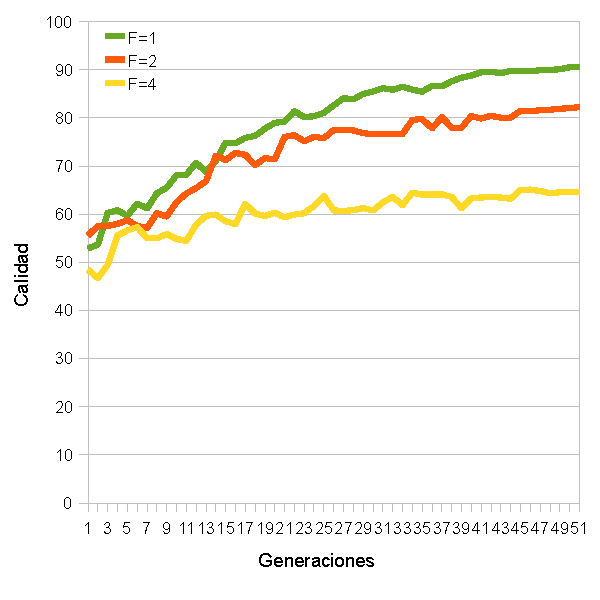
\includegraphics[width=0.4\textwidth]{figs/graphs/FactorFitnessBest}
	\label{subfig:p-factorfitness-best}
  }                
  \subfloat[Calidad media de la población]{
  	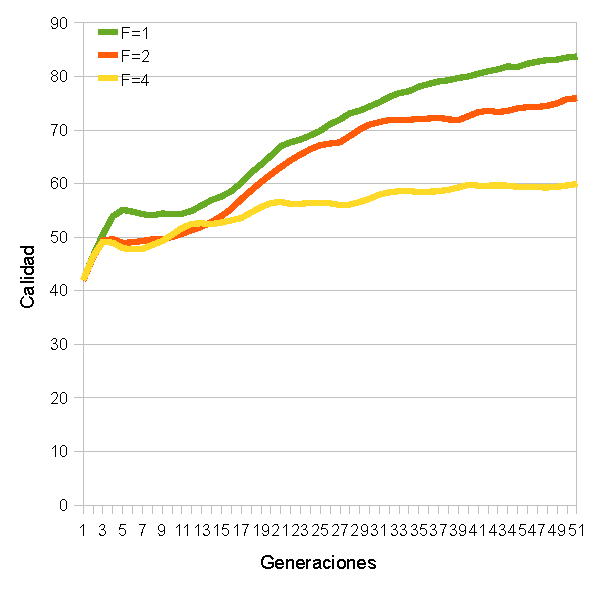
\includegraphics[width=0.4\textwidth]{figs/graphs/FactorFitnessMean}
	\label{subfig:p-factorfitness-mean}%
  }
  \quad
  \subfloat[Número de nodos medio de la población]{
  	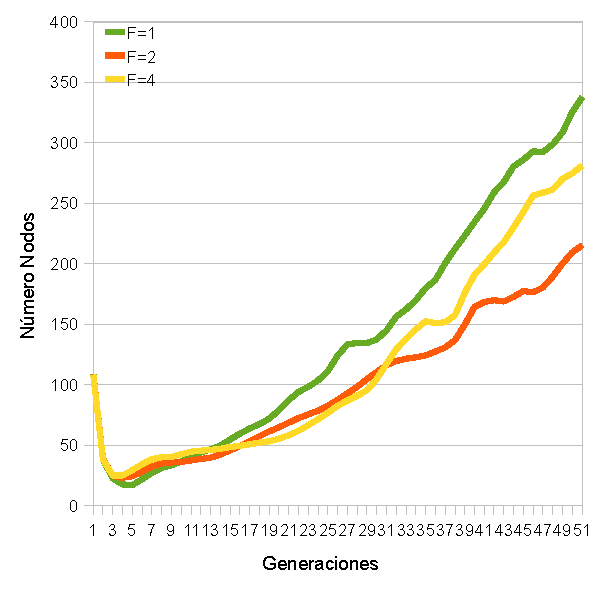
\includegraphics[width=0.4\textwidth]{figs/graphs/FactorFitnessNodes}
	\label{subfig:p-factorfitness-nodes}%
  }
  \subfloat[Tiempo de las ejecuciones]{
  	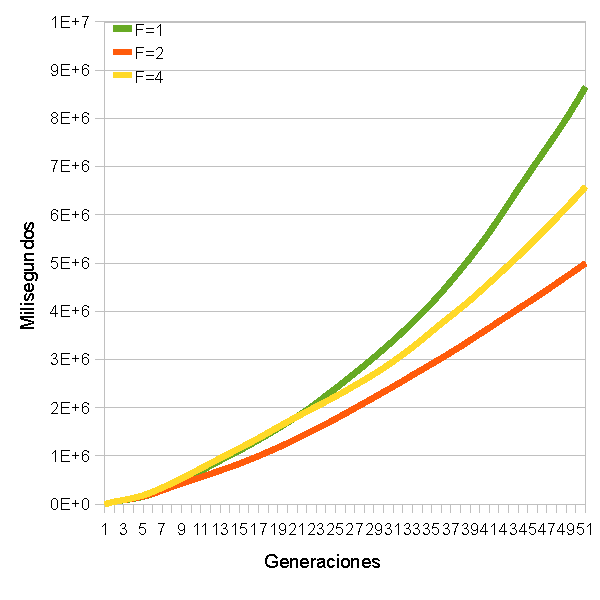
\includegraphics[width=0.4\textwidth]{figs/graphs/FactorFitnessTime}
	\label{subfig:p-factorfitness-time}%
  }
  \centering
\caption{Factor fitness ($F$)}
\label{fig:p-factorfitness}
\end{figure}

